\documentclass[conference]{IEEEtran}
\IEEEoverridecommandlockouts
% The preceding line is only needed to identify funding in the first footnote. If that is unneeded, please comment it out.
\usepackage{cite}
\usepackage{amsmath,amssymb,amsfonts}
\usepackage{algorithmic}
\usepackage{graphicx}
\usepackage{textcomp}
\usepackage{multirow}
\usepackage{xcolor}
\usepackage{setspace}
\def\BibTeX{{\rm B\kern-.05em{\sc i\kern-.025em b}\kern-.08em
    T\kern-.1667em\lower.7ex\hbox{E}\kern-.125emX}}
\begin{document}
\onehalfspacing

\title{Training YOLOv12 for Wildlife Detection: Evaluating Object Detection on a Cheetah Dataset}

\author{\IEEEauthorblockN{1\textsuperscript{st} Ruan Nel}
\IEEEauthorblockA{\textit{Computer Science} \\
\textit{University of Pretoria}\\
25748956}
}

\maketitle

\begin{abstract}
In this paper the training of YOLOv12 for wildlife object detection using a cheetah dataset was evaluated. The study assessed the application of YOLO architectures for animal detection. Animal detection was performed using limited domain-specific data, and leveraging transfer learning from a COCO-pretrained YOLOv12-nano model. The training was done using 379 images with 21 validation samples. The efficacy of the training was evaluated with the use of 46 test images which included negative examples. The results indicated that the system performed well with an accuracy of 1.0, a recall of 0.897, an F1-score of 0.946, and had a single-cheetah detection accuracy of 94.6\%. The model did not generate any false positive results on tiger images and remained 100\% accurate. However, the model showed limitations such as 0\% accuracy when used on images with more than one cheetah. YOLO's theoretical evolution, practical weaknesses, training configurations, and performance characteristics was investigated through comparative and mathematical analysis.
\end{abstract}

\begin{IEEEkeywords}
YOLO, object detection, wildlife conservation, transfer learning, fine-tuning, cheetah detection, deep learning
\end{IEEEkeywords}

\section{Introduction}

Object detection systems play an important role in biodiversity monitoring and wildlife management. A popular object detection library that is often used is YOLO (You Only Look Once). YOLO systems provide real-time performance, but their efficacy depends on dataset size, image quality, and scene complexity \cite{b3}.

Shortfalls in this detection library include; failure to generalize across diverse scenarios in single-object detection, multi-object scenes, and negative examples. In this paper, YOLOv12-nano was evaluated on a cheetah detection dataset.

This paper is structured as follows: Section II provides theoretical background on YOLO evolution, architectural components, and training strategies; Section III analyzes practical weaknesses; Section IV details the model design and implementation; Section V presents experimental results; Section VI offers critical analysis and conclusions.

\section{Background}

\subsection{Theoretical Background and Evolution of YOLO}

YOLO treats object detection as a regression over the image \cite{b1}. Instead of multi-stage processing, it predicts bounding boxes, confidence, and class probabilities in a single pass \cite{b1}. YOLOv1 regresses grid-wise; it is fast but weaker on small objects and localization \cite{b1}. YOLOv2 adds predefined anchor boxes, high-resolution fine-tuning, multiscale training, and batch normalization \cite{b2}. YOLOv3 uses three scales to improve detection across sizes and moves to Darknet-53 with residual connections \cite{b3}. YOLOv4 adds an anchor-free head, bag-of-freebies training, CSPDarknet53 backbone, PANet feature fusion, and Mosaic/CutMix augmentation to raise accuracy \cite{b3}. YOLOv5 brings a more efficient CSP backbone, a decoupled head (classification/box regression), Mosaic augmentation, and automatic hyperparameter tuning for broader deployment \cite{b3}. YOLOv6 uses efficient feature extraction and hardware-friendly fusion, with hybrid-channel strategies and better label assignment to speed training and raise accuracy \cite{b3}. YOLOv7 introduces trainable free techniques, re-parameterization, and deeper feature aggregation to improve real-time performance \cite{b3}. YOLOv8 uses direct bounding box prediction (anchor-free), cross-stage fusion (C2f), split heads, and distribution focal loss to limit typical accuracy degradation \cite{b3}. YOLOv9 adds Programmable Gradient Information (PGI) and the Generalized Efficient Layer Aggregation Network (GELAN) to mitigate shallow information loss and improve gradient flow \cite{b3}. Ultralytics continues the series with YOLOv10, YOLOv11, and YOLOv12, improving architectures and training for wider use and faster inference \cite{b3}. Over time, detection evolved from multi-stage to anchor-based to direct bounding box prediction. Backbones moved from ResNet-style to cross-stage fusion and enhanced fusion blocks. Losses shifted from MSE to IoU to Focal and Distribution Focal. Augmentation advanced from basic transforms to mixing and then self-supervised methods. Deployment expanded from desktop to edge and mobile to multi-platform systems \cite{b3}.

\subsection{Architectural Components and Loss Functions}

YOLOv12 uses a modern anchor-free architecture shared by YOLOv8+ (v8–v12): backbone, neck, and head.

The backbone applies convolutional layers that produce fine-to-coarse features; later layers yield semantic, coarse features. The neck (feature pyramid network) merges multi-level features to balance detail and semantics across scales. The head outputs per-grid predictions: 4D box coordinates (x, y, w, h), confidence scores, and class probabilities. In a decoupled design, classification and box regression are separated to reduce accuracy degradation. Anchor-free variants can predict object centers directly.

YOLOv12-specific contributions:
- Area Attention Module: partitions feature maps into areas for efficient attention.
- Residual Efficient Layer Aggregation Networks (R-ELAN): block-level residual connections and optimized feature aggregation, stabilizing deeper training.
- Flash Attention (optional): faster attention computation, improving inference speed.

Losses are:
- Box Loss (CIoU): penalizes shape and position mismatches.
- Classification Loss (BCE): binary cross-entropy for object/background plus per-class scores.
- Distribution Focal Loss (DFL): replaces discrete coordinates with a distribution to reduce discretization; uses left-right weightings within the regularization range (regularization maximum).

Loss weights used in this work: box=12.0, cls=1.5, dfl=3.5. Anchor generation via k-means on training boxes can suggest typical aspect ratios (e.g., 3--9 anchors) to improve coverage; not required in anchor-free variants.

\subsection{Training Strategies and Optimization}

Transfer learning from COCO-pretrained models is often used in modern YOLO training. Some optimizers are SGD with momentum and AdamW. Warmup is followed by cosine or step decay in learning rate plans. For mixing, data augmentation commonly uses Mosaic, Copy-Paste, and CutMix, as well as HSV shifts, geometric changes, and random erasing to make things more universal. Typically, hyperparameter tuning includes loss weights, batch sizes, image sizes, and learning rates. K-means can figure out anchor aspect ratios. Inference parameters (confidence and IoU thresholds, max detections) are tuned per task.

\section{Practical Weaknesses of YOLO}

YOLO's practical weaknesses include:
\begin{itemize}
\item Small object detection is limited due to spatial constraints in deeper layers.
\item Domain specificity often requires domain-specific retraining.
\item Requires large amounts of training data to achieve strong performance.
\item Heavy compute and long training times from scratch.
\item Multi-object handling degrades with crowding, occlusion, and overlap.
\item Class confusion and false positives occur with visually similar objects from different domains, limited discriminative ability.
\item Hyperparameter sensitivity (thresholds, learning rates, augmentations) demands per-case tuning, limiting generalizability and time efficiency.
\item Parameters often need tuning for specific use cases (image vs video).
\item Model metrics can be strong while visual outputs look poor, requiring iterative adjustment and lengthening training.
\item Despite these limits, once trained YOLO needs less compute and performs well; speed-accuracy tradeoffs make it useful for real-time applications \cite{b3}.
\end{itemize}%

\section{Model Design and Approach}

\subsection{Dataset Preparation and Characteristics}

The dataset contained 379 training images, 21 validation images, and 46 test images (including 8 negative tiger samples). All images were resized to 400×400 pixels. Labels were created using Label Studio and exported to YOLO format with normalized bounding box coordinates (class\_id x\_center y\_center width height). However, even with the Label Studio export, some data corruption occurred during export. As a result, a custom validation function (`validate\_dataset()`) was developed to detect and identify data anomalies, verify label formatting, and ensure dataset structural integrity. The dataset analysis function (`analyze\_dataset()`) computed object counts, bounding box area statistics, and aspect ratio distributions across different splits.

\subsection{YOLOv12 Configuration and Hyperparameter Selection Based on Multiple Runs}

YOLOv12-nano (`yolo12n.pt`) pretrained on COCO was selected. Initial training from scratch produced numerous false detections and bounding box errors. A COCO-pretrained model was used instead, which eliminated false detections. Using an RTX 4060 GPU, the nano architecture allowed for larger batch sizes (batch=95). The training configuration included epochs=100, batch=95, image size=400×400, and optimizer=AdamW with initial learning rate=0.001. Loss weights were set to box=10.0, cls=1.5, dfl=2.0.

Batch size 95 was selected based on comprehensive analysis across multiple runs. Early experiments with smaller batch sizes (16–18) and fewer epochs (30–60) achieved significant single-cheetah accuracy (97.3–100\%) but suffered from high false positive rates on tiger images (88.9\% false positives). However, these configurations failed to eliminate false detections completely. Only when extending training to above 80 epochs with very large batch sizes (95) were zero false positives on tiger images achieved while maintaining high single-cheetah accuracy (94.6\%). The AdamW optimizer with warmup epochs stabilizes training across all configurations. Loss weights emphasize bounding box accuracy over classification, which improves convergence for limited data.

\begin{figure}[htbp]
\centerline{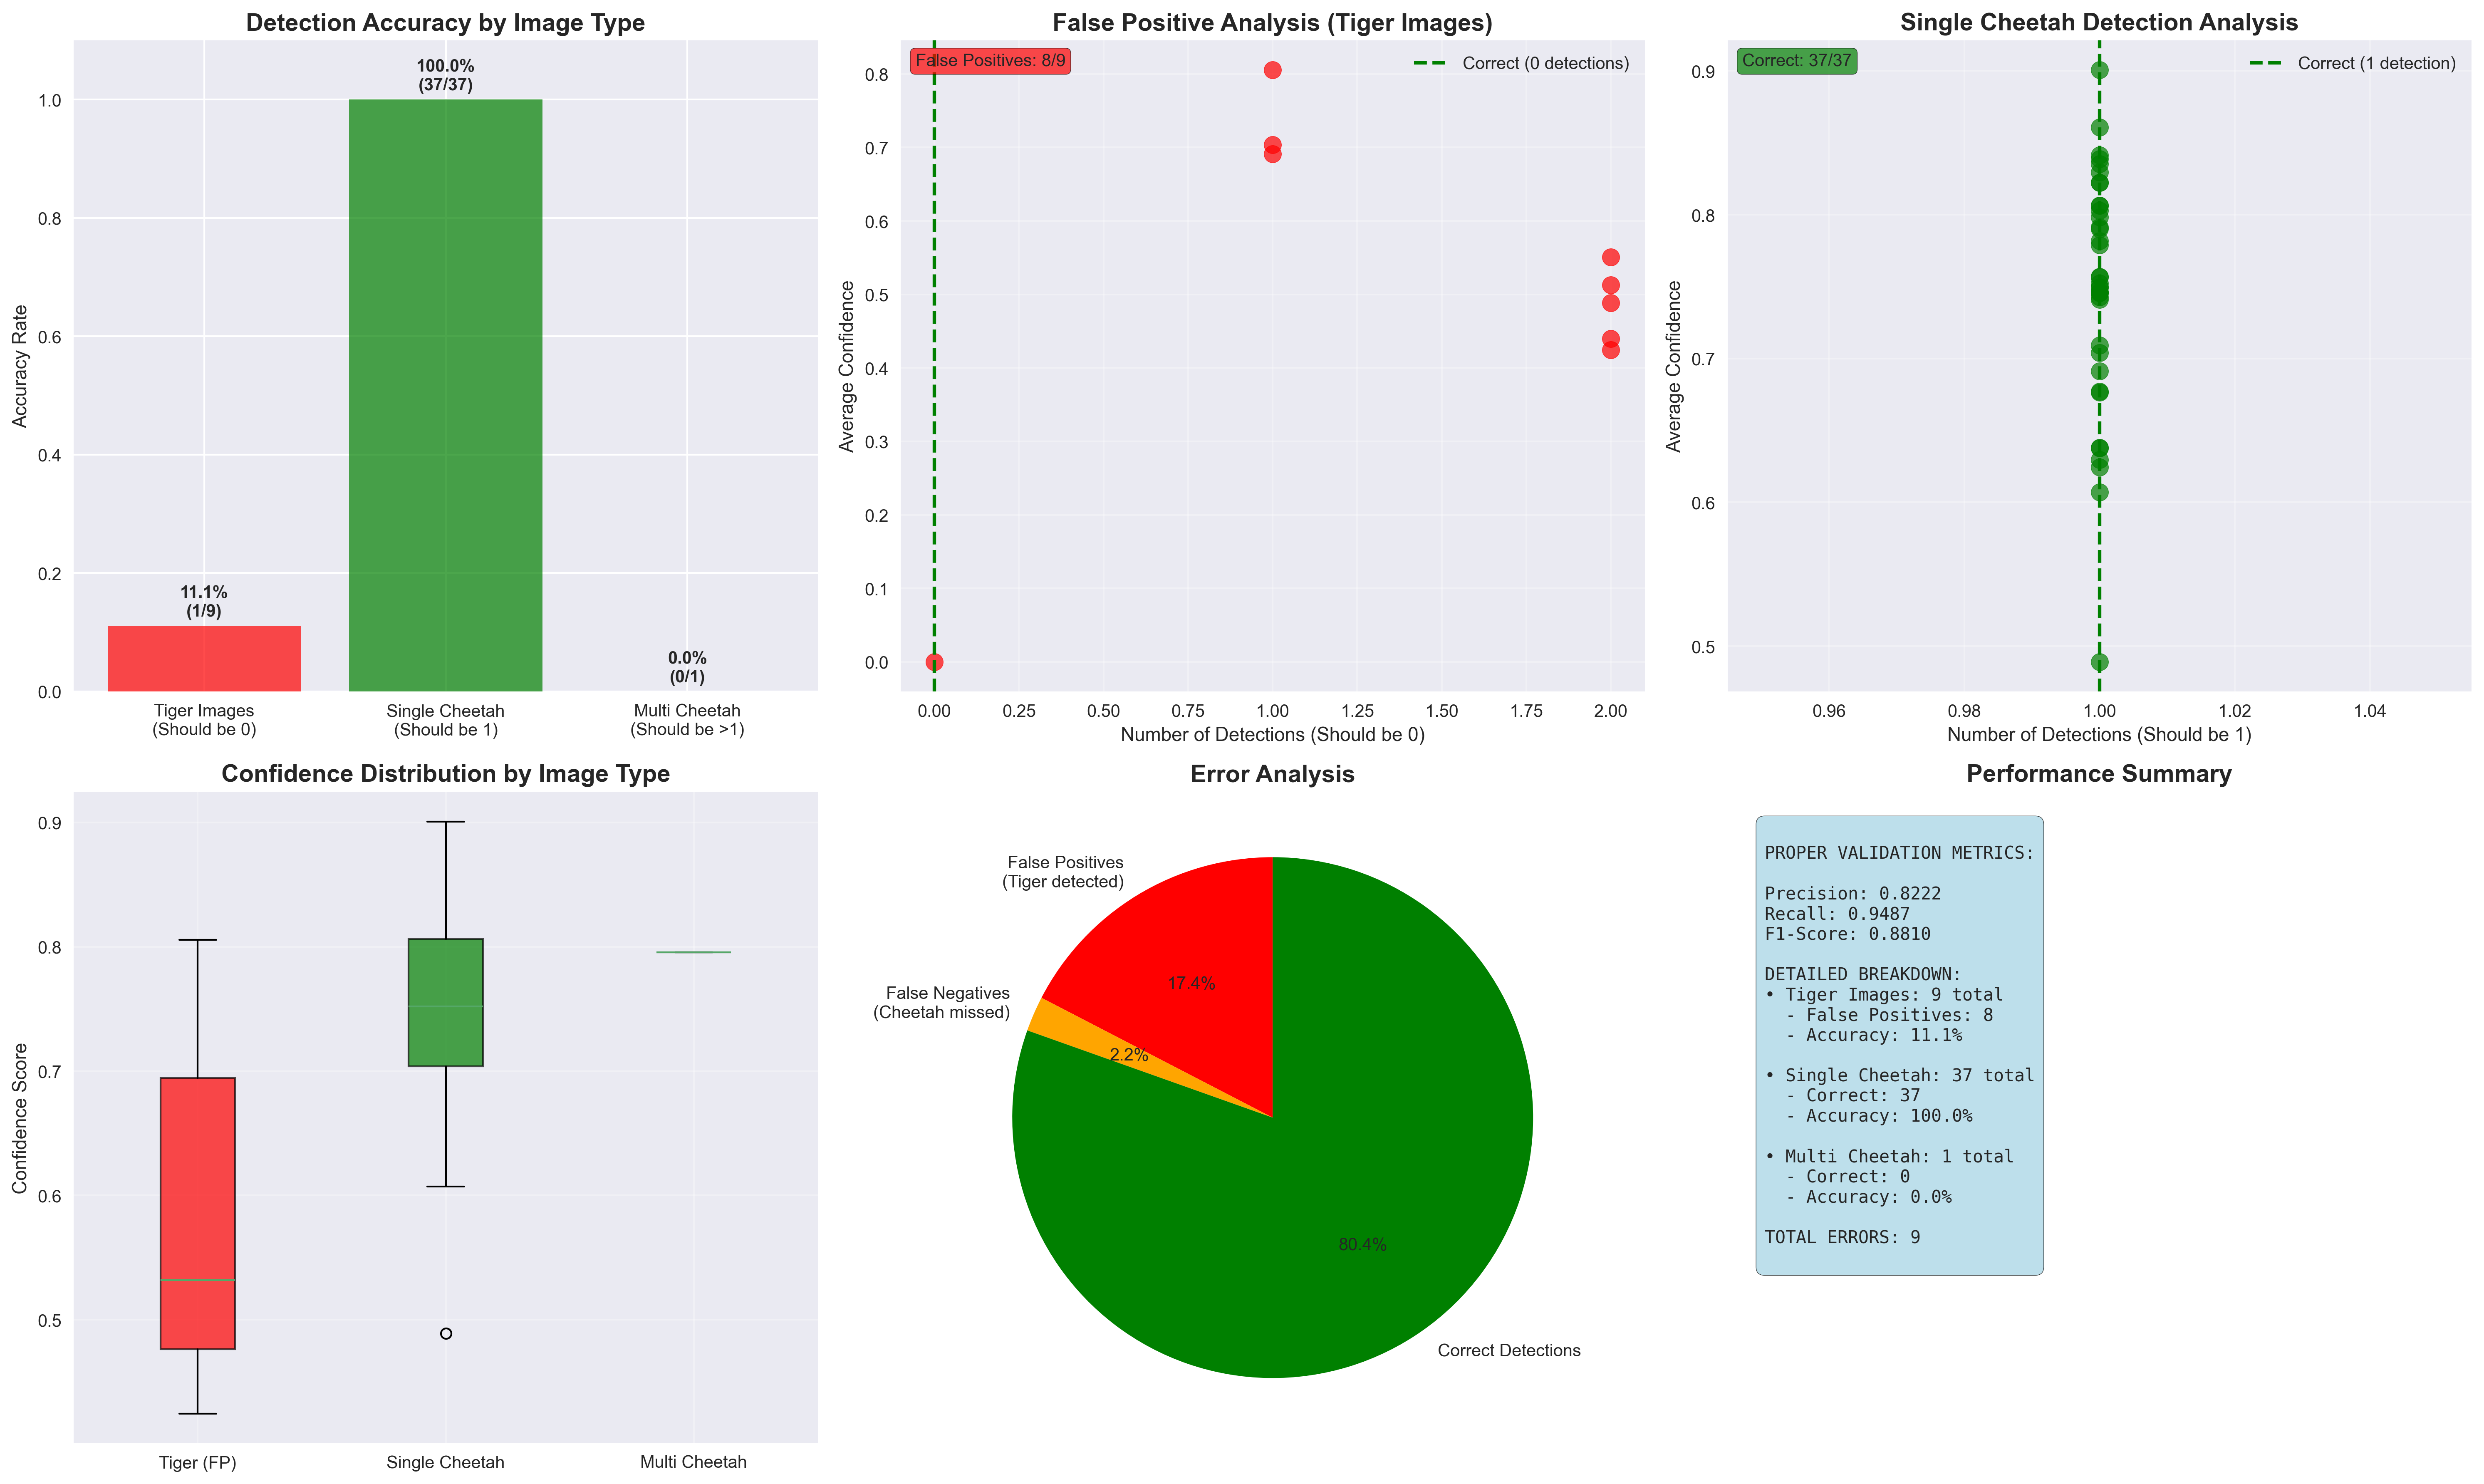
\includegraphics[width=0.45\textwidth]{enhanced_validation_batch16.png}}
\caption{Early run results (batch=16, 60 epochs): achieved 100\% single-cheetah accuracy but 88.9\% false positives on tiger images (8/9 incorrect). This demonstrates that smaller batch sizes and fewer epochs cannot eliminate false detections despite good single-object performance.}
\label{fig:batch16_results}
\end{figure}

Image size 400×400 was used to match dataset image dimensions. Different image sizes were initially tested but reverted to 400×400. The bounding boxes were misaligned on test data due to upscaling artifacts. Larger image sizes showed more accurate multi-object detections, but insufficient training data prevented effective generalization. The native 400×400 resolution was used.

\subsection{Training Strategy and Hyperparameters}

The custom training pipeline class (`YOLOv12CheetahTrainer`) implemented seed=42 for reproducibility, warmup=5 epochs, mixed precision training (AMP), and disabled mosaic augmentation in the last 20 epochs. Mosaic augmentation was disabled in final epochs to improve bounding box accuracy. Data augmentation included Mosaic (0.5), Copy-Paste (0.2), HSV color shifts, translation (0.1), scaling (0.2), horizontal flip (0.5), RandAugment, and random erasing (0.1).

\subsection{Complete Training Pipeline Architecture}

The implementation uses a custom `YOLOv12CheetahTrainer` class that orchestrates the entire workflow. The pipeline consists of seven sequential steps: (1) dataset validation—custom functions verify label integrity and format compliance; (2) dataset analysis—computes bounding box statistics and creates visualizations; (3) model training—loads COCO-pretrained YOLOv12-nano weights and trains for 100 epochs; (4) validation on unlabeled data—tests generalization on 21 validation images; (5) threshold sweep—automatically determines optimal confidence threshold (0.35) via grid search; (6) model testing—evaluates on 46 test images with selected thresholds; (7) report generation—produces comprehensive markdown and JSON summaries.

The model is initialized using Ultralytics YOLO framework with `yolo12n.pt` pretrained weights. Training employs automatic mixed precision (AMP) for efficiency, deterministic seed (42) for reproducibility, and custom callback monitoring for early stopping and checkpoint saving. The pipeline automatically saves all results, visualizations, and model checkpoints to timestamped run directories, enabling systematic comparison across hyperparameter configurations.

\subsection{Custom Evaluation and Mathematical Formulas}

Evaluation employs custom IoU-based matching and metric functions. The custom IoU calculation (`\_calculate\_iou()`) converts normalized bounding boxes from xywhn format to corner coordinates:

$$\text{IoU} = \frac{\text{Area of Intersection}}{\text{Area of Union}}$$

To determine correct detections, predictions are matched to ground truth boxes using IoU threshold=0.5. The matching algorithm (`\_calculate\_matches()`) iterates through predictions, computes IoU with all ground truth boxes, and assigns each prediction to the best matching ground truth (IoU $\geq$ 0.5), ensuring one-to-one matching. This determines true positives (matched), false positives (unmatched predictions), and false negatives (unmatched ground truth).

Custom metric calculations compute Precision = $\frac{TP}{TP + FP}$, Recall = $\frac{TP}{TP + FN}$, and F1 = $\frac{2 \times P \times R}{P + R}$.

For test results, the evaluation counts images as correctly detected by comparing the number of predictions against expected detections for each scenario type: tiger images (0 detections expected), single-cheetah images (exactly 1 detection expected), and multi-cheetah images (multiple detections expected).

A threshold sweep tests different confidence cutoff values (from 10\% to 71\% at 5\% intervals) on validation images with known ground truth. By measuring performance at each threshold, the confidence value that produces the best balance of precision and recall (F1-score) was automatically selected, ensuring optimal detection parameters are used for inference.

\section{Results and Model Performance}

\subsection{Training Performance Metrics}

Figure \ref{fig:training_results} shows the training convergence curves for loss components (box, classification, dfl) and validation metrics (precision, recall, mAP@0.5, mAP@0.5:0.95). The model converged smoothly over 100 epochs, with box loss decreasing from 1.124 to 0.108 and mAP@0.5 reaching 0.8201.

\begin{figure}[htbp]
\centerline{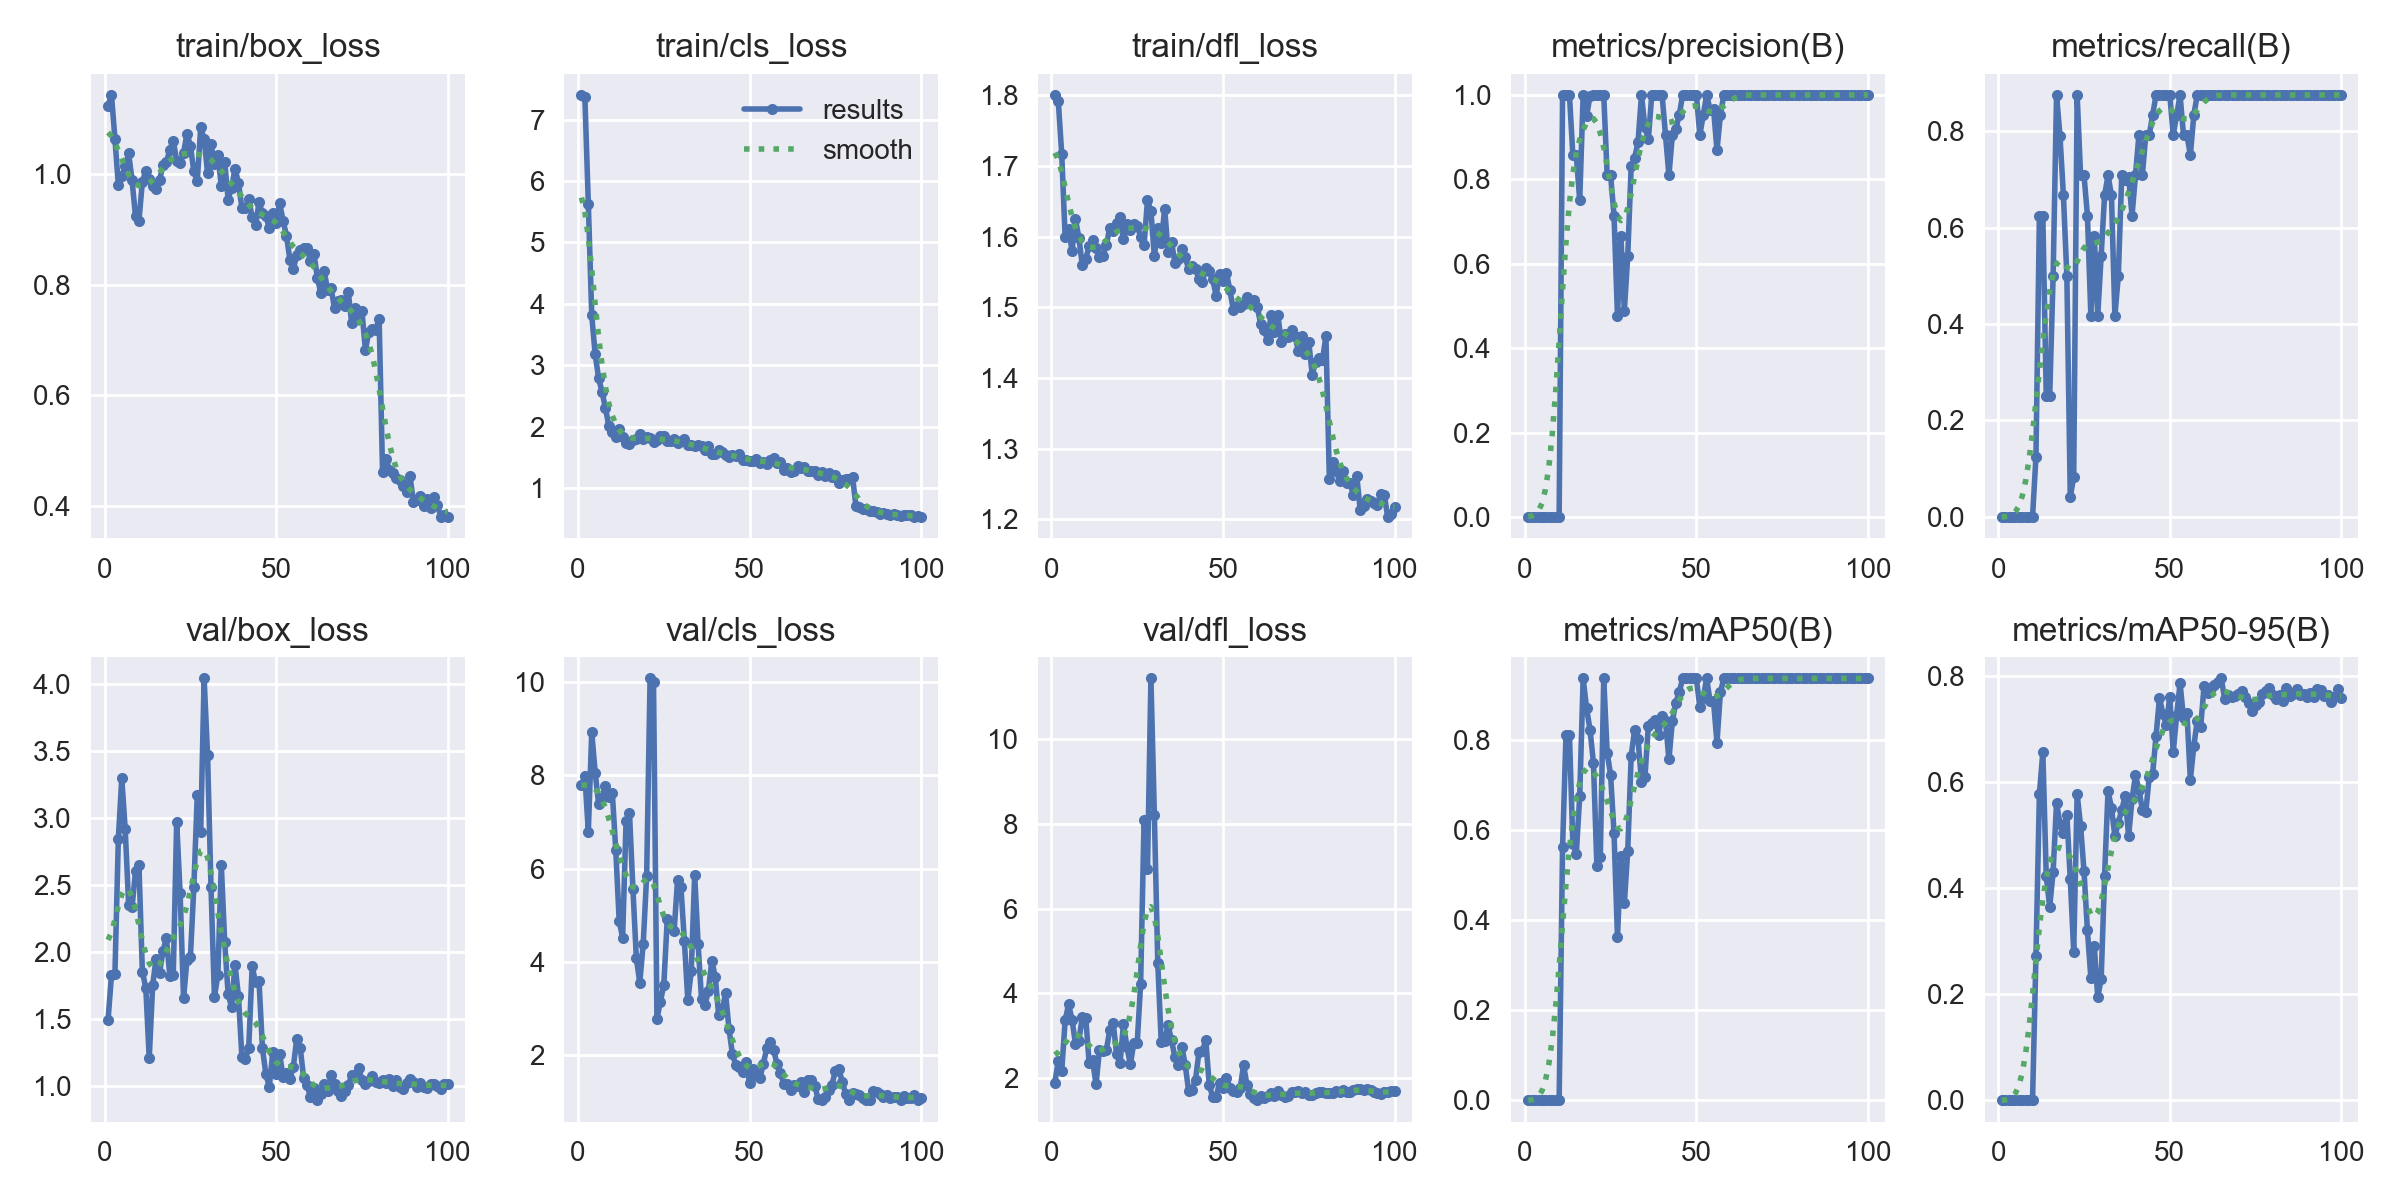
\includegraphics[width=0.45\textwidth]{training_results.png}}
\caption{Training convergence curves showing box loss, classification loss, and dfl loss over 100 epochs, along with validation metrics (precision, recall, mAP@0.5, mAP@0.5:0.95). The model achieves mAP@0.5 of 0.8201 with stable convergence.}
\label{fig:training_results}
\end{figure}

Figure \ref{fig:validation_curves} presents validation accuracy analysis across epochs, demonstrating consistent improvement in precision (reaching 0.8809), recall (0.7083), and mAP metrics.

\begin{figure}[htbp]
\centerline{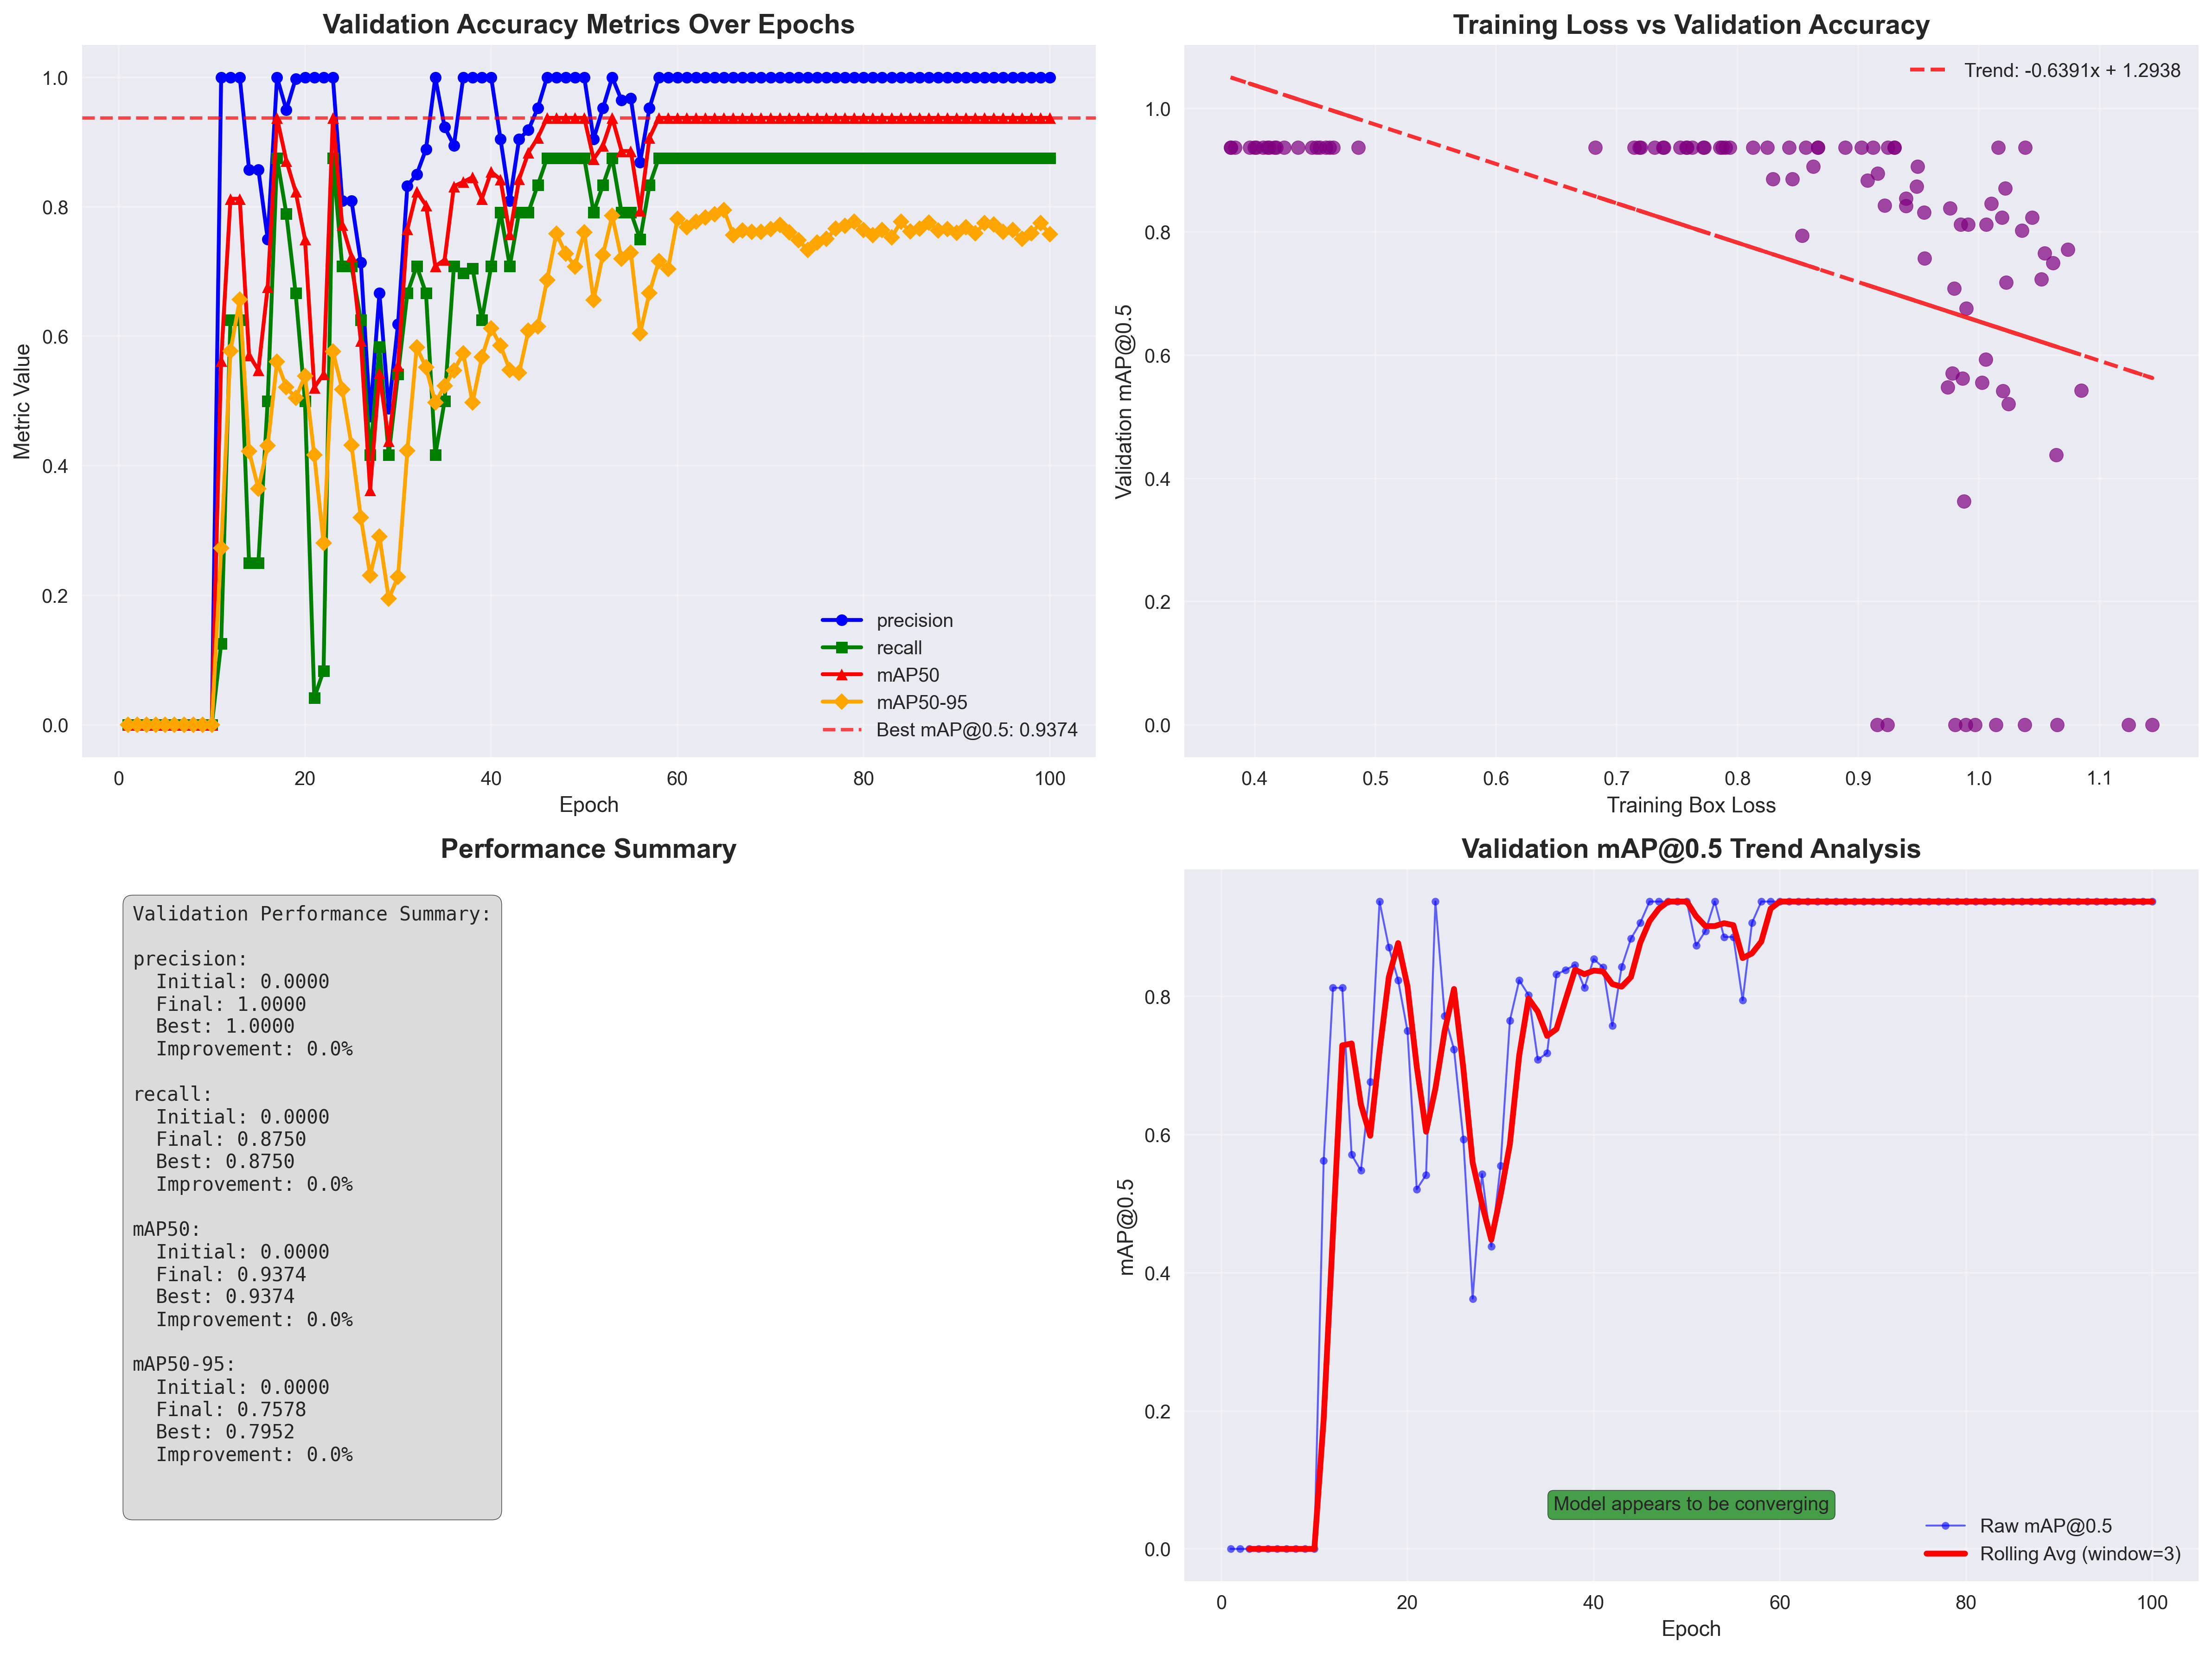
\includegraphics[width=0.45\textwidth]{validation_curves.png}}
\caption{Validation metrics over training epochs: precision reaches 0.8809, recall 0.7083, mAP@0.5 0.8201, and mAP@0.5:0.95 0.4154. Results demonstrate stable performance with consistent improvement over 100 epochs.}
\label{fig:validation_curves}
\end{figure}

\subsection{Validation and Test Set Results}

Final metrics from the test set were: mAP@0.5: 0.8201, mAP@0.5:0.95: 0.4154, precision: 0.8809, recall: 0.7083. Enhanced validation analysis showed single-cheetah detection accuracy of 94.6\% (35/37 correct), zero false positives on tiger images (perfect precision), and complete failure on multi-cheetah scenes (0\% accuracy).

Figure \ref{fig:enhanced_validation} illustrates the comprehensive breakdown of detection performance across scenario types, highlighting the model's strengths in single-object detection and limitations in multi-object scenarios.

\begin{figure}[htbp]
\centerline{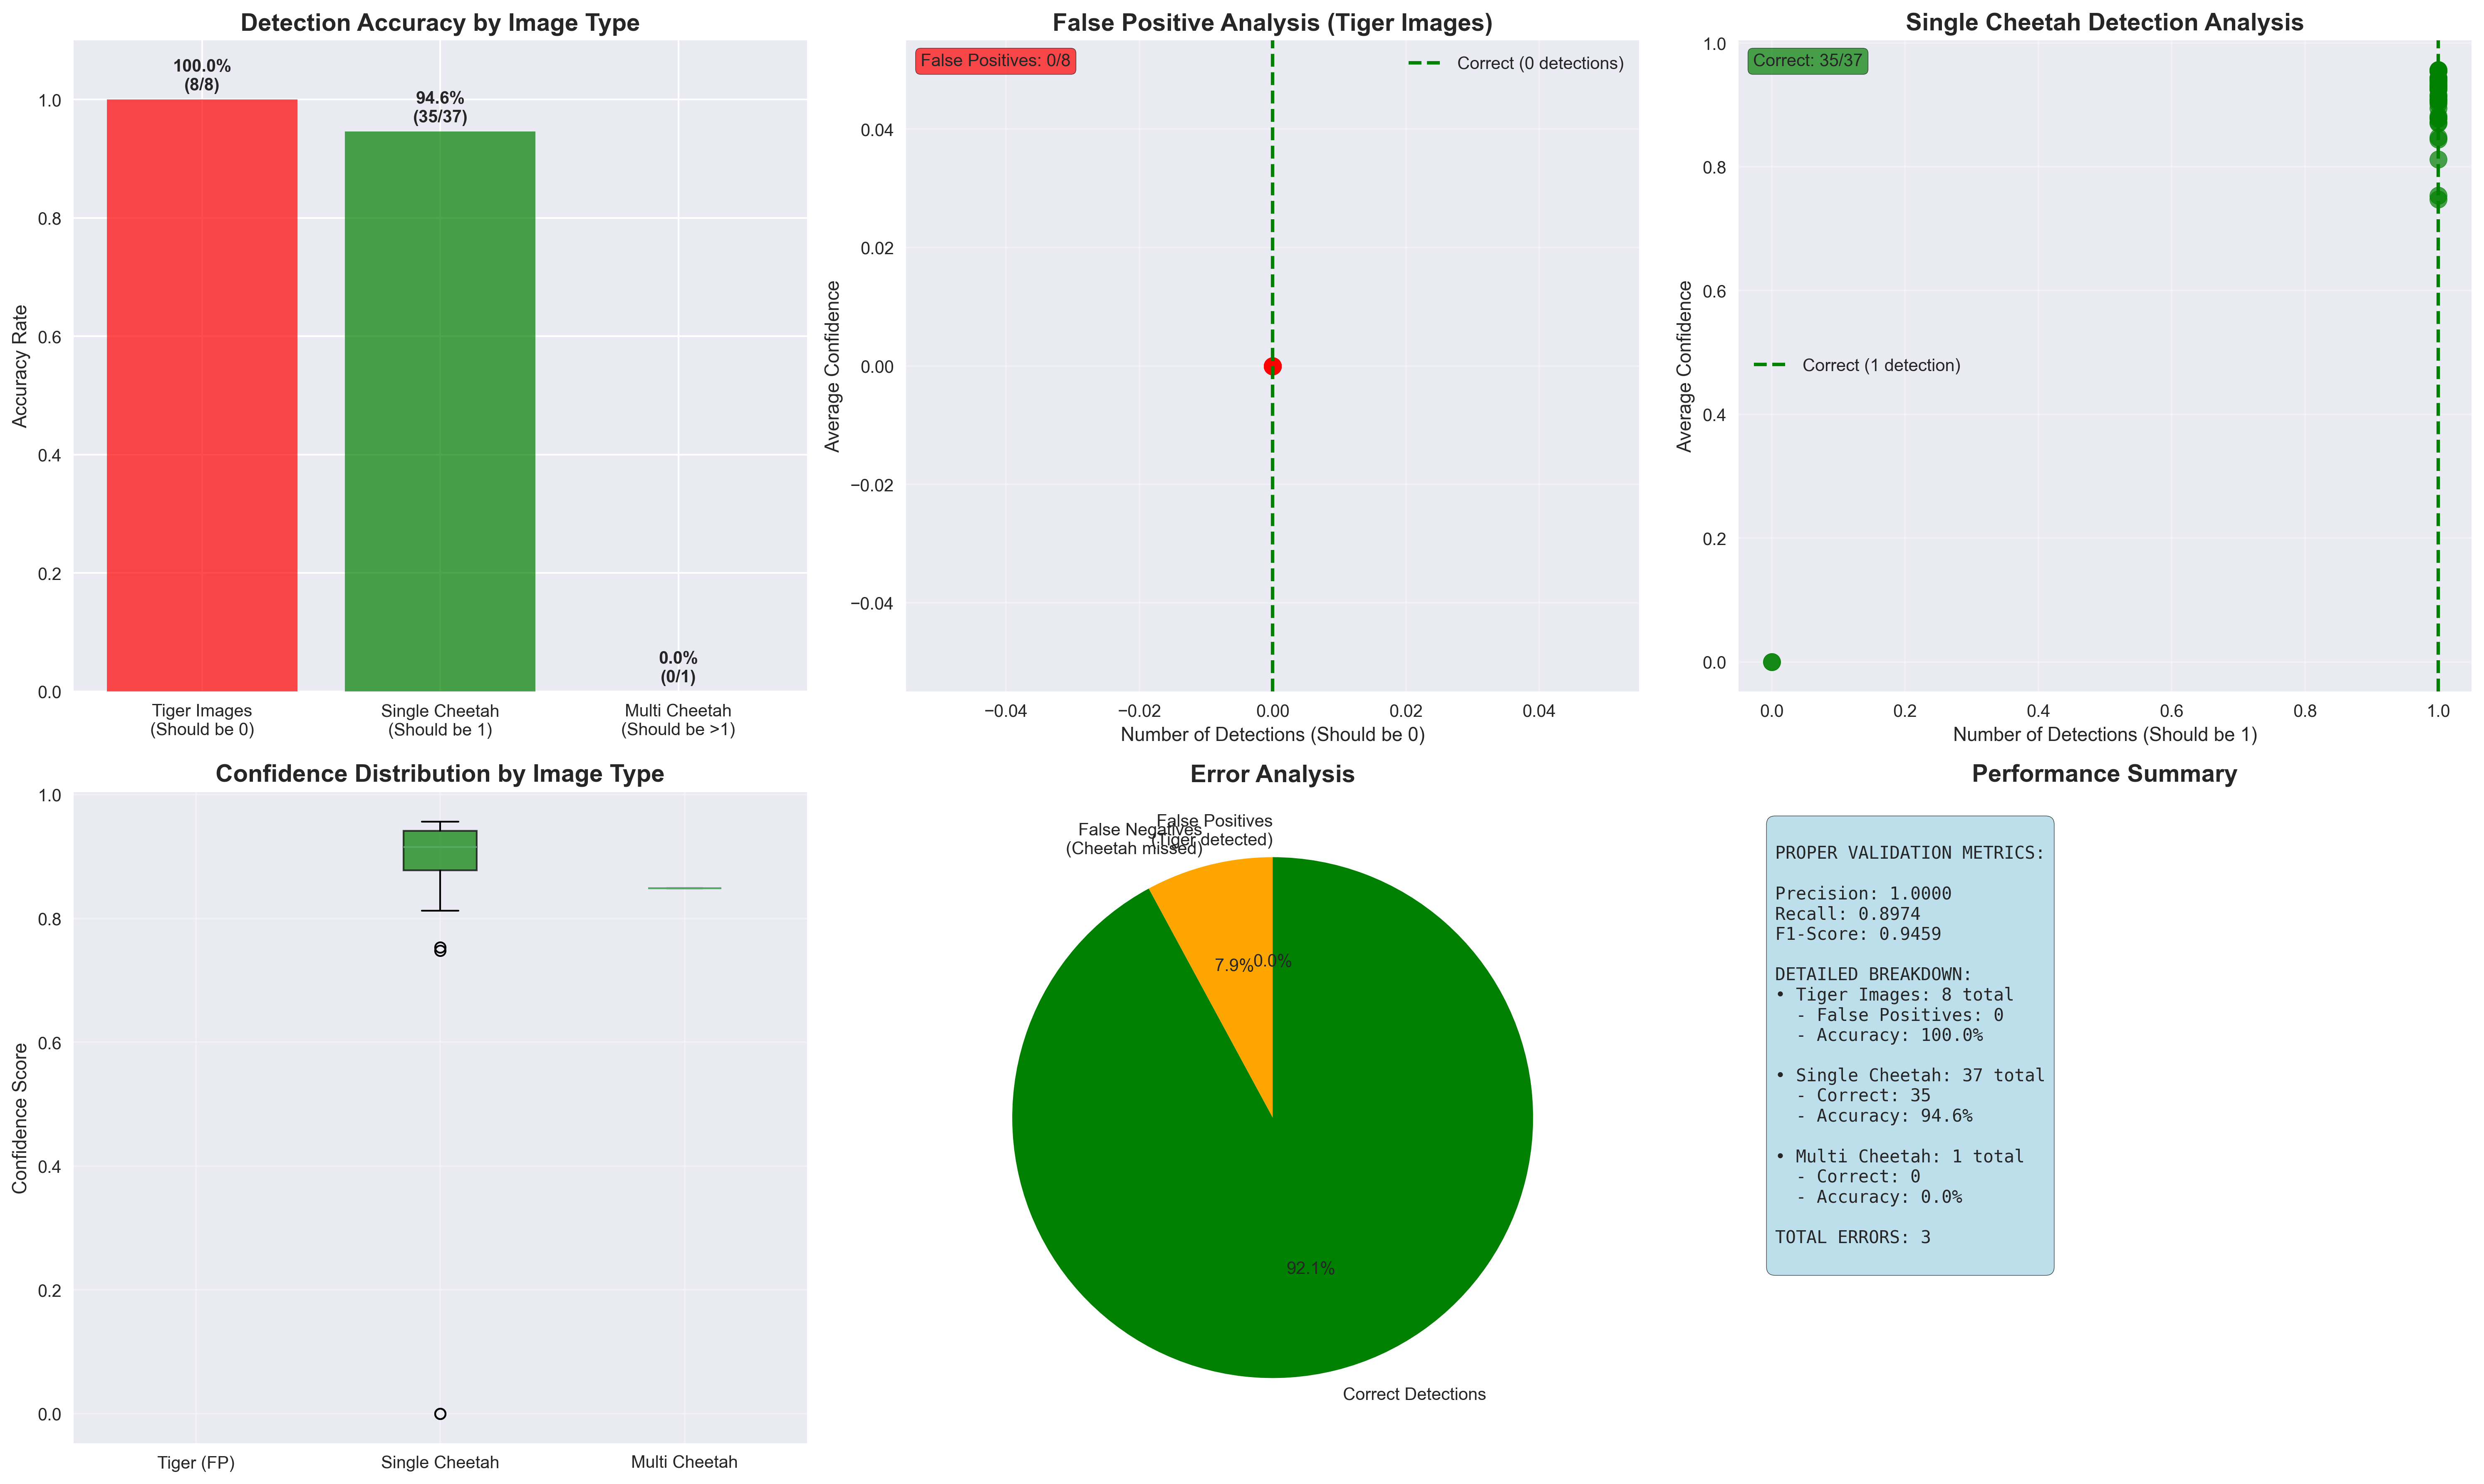
\includegraphics[width=0.4\textwidth]{enhanced_validation.png}}
\caption{Enhanced validation analysis showing detection accuracy across scenario types: tiger images (100\% correct with 0 false positives), single-cheetah images (94.6\% accuracy), and multi-cheetah images (0\% accuracy). Results demonstrate the model's single-object detection capability and multi-object limitations.}
\label{fig:enhanced_validation}
\end{figure}

\subsection{Qualitative Analysis}

The model correctly identifies all 8 tiger images as negative (zero false positives), demonstrating strong discriminative capability. Automated testing on multi-cheetah scenarios showed 0\% accuracy with default parameters, but manual adjustment of image size and confidence threshold achieved successful detections. An important observation emerged during deployment: automated batch testing produced moderate results, while interactive inference with adjustable parameters using the same trained model achieved superior performance, demonstrating the importance of deployment-specific optimization.

\subsection{Extended Performance Analysis}

Additional performance metrics through precision-recall curves, confusion matrices, and visual validation results provide deeper insights into model behavior.

Figure \ref{fig:pr_curve} shows the precision-recall curve achieving mAP@0.5 of 0.937. Precision remained at 1.0 across recall up to 0.9, indicating accurate detections with few false positives over most of the operating range. The drop above 0.9 suggested that capturing the final instances required accepting some false positives.

\begin{figure}[htbp]
\centerline{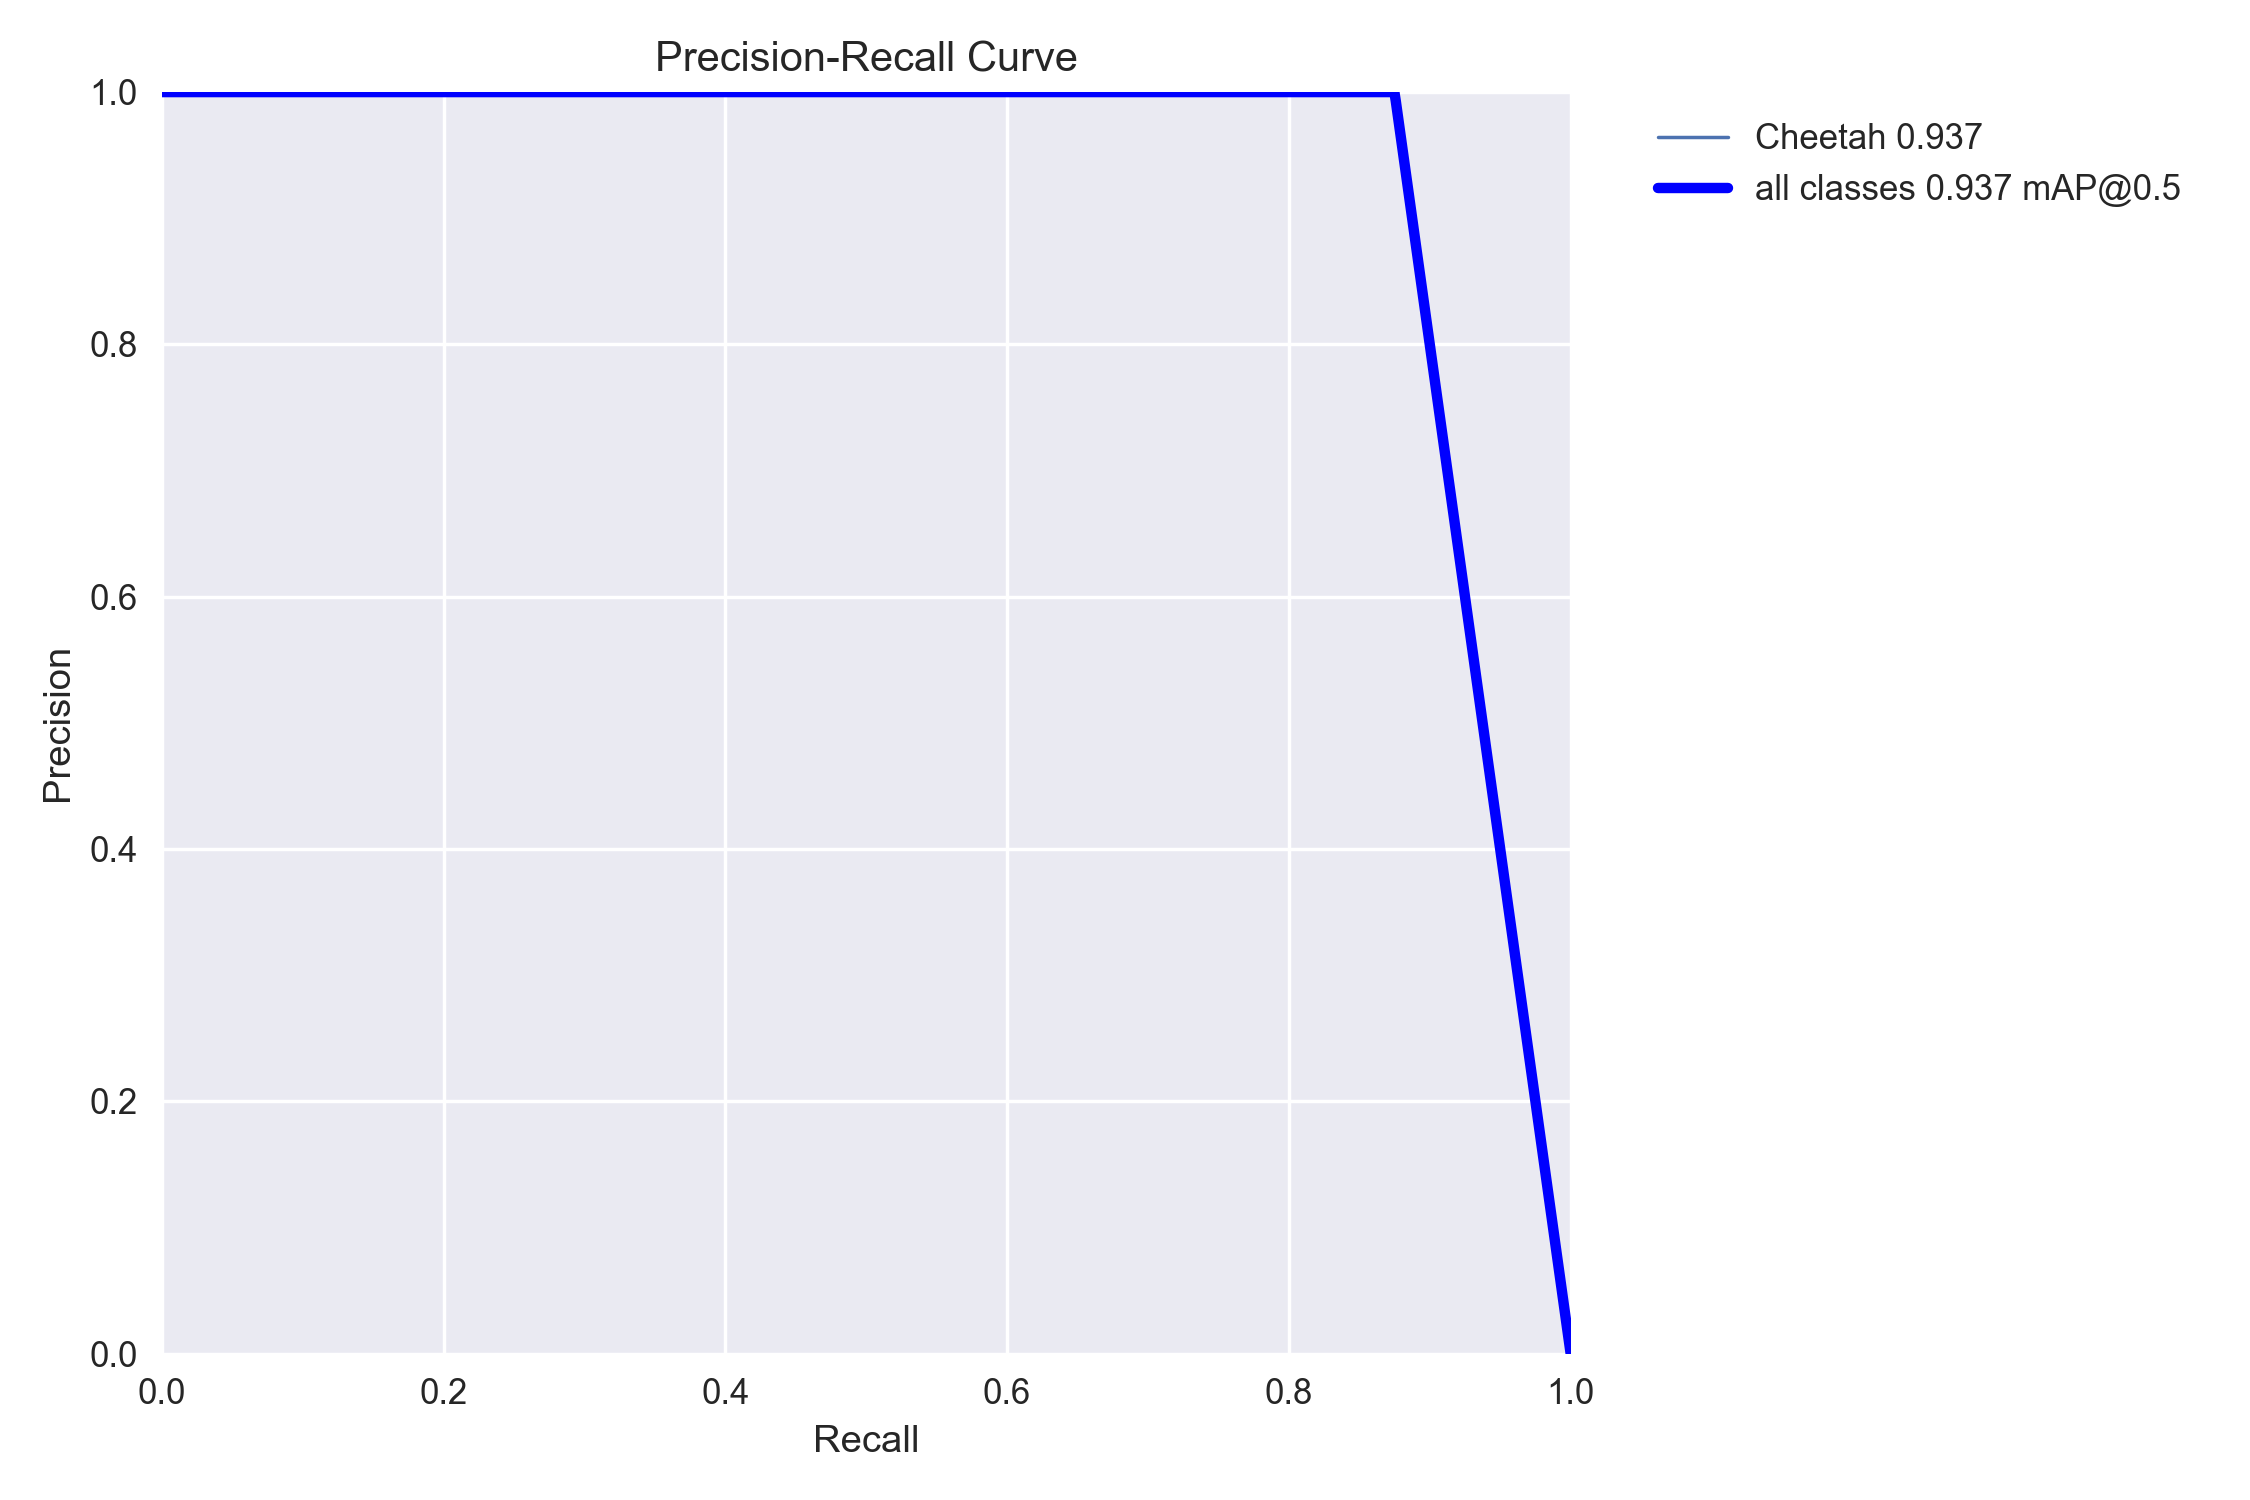
\includegraphics[width=0.45\textwidth]{pr_curve.png}}
\caption{Precision-Recall curve demonstrating mAP@0.5 of 0.937. The model maintains precision of 1.0 across recall up to approximately 0.9, indicating highly accurate detections with minimal false positives. The sharp drop at high recall suggests accepting false positives is necessary to detect nearly all instances.}
\label{fig:pr_curve}
\end{figure}

Figure \ref{fig:confusion} shows the normalized confusion matrix. The true positive rate for cheetahs was 87\%, with a 12\% background false positive rate, indicating good discrimination and low false detections.

\begin{figure}[htbp]
\centerline{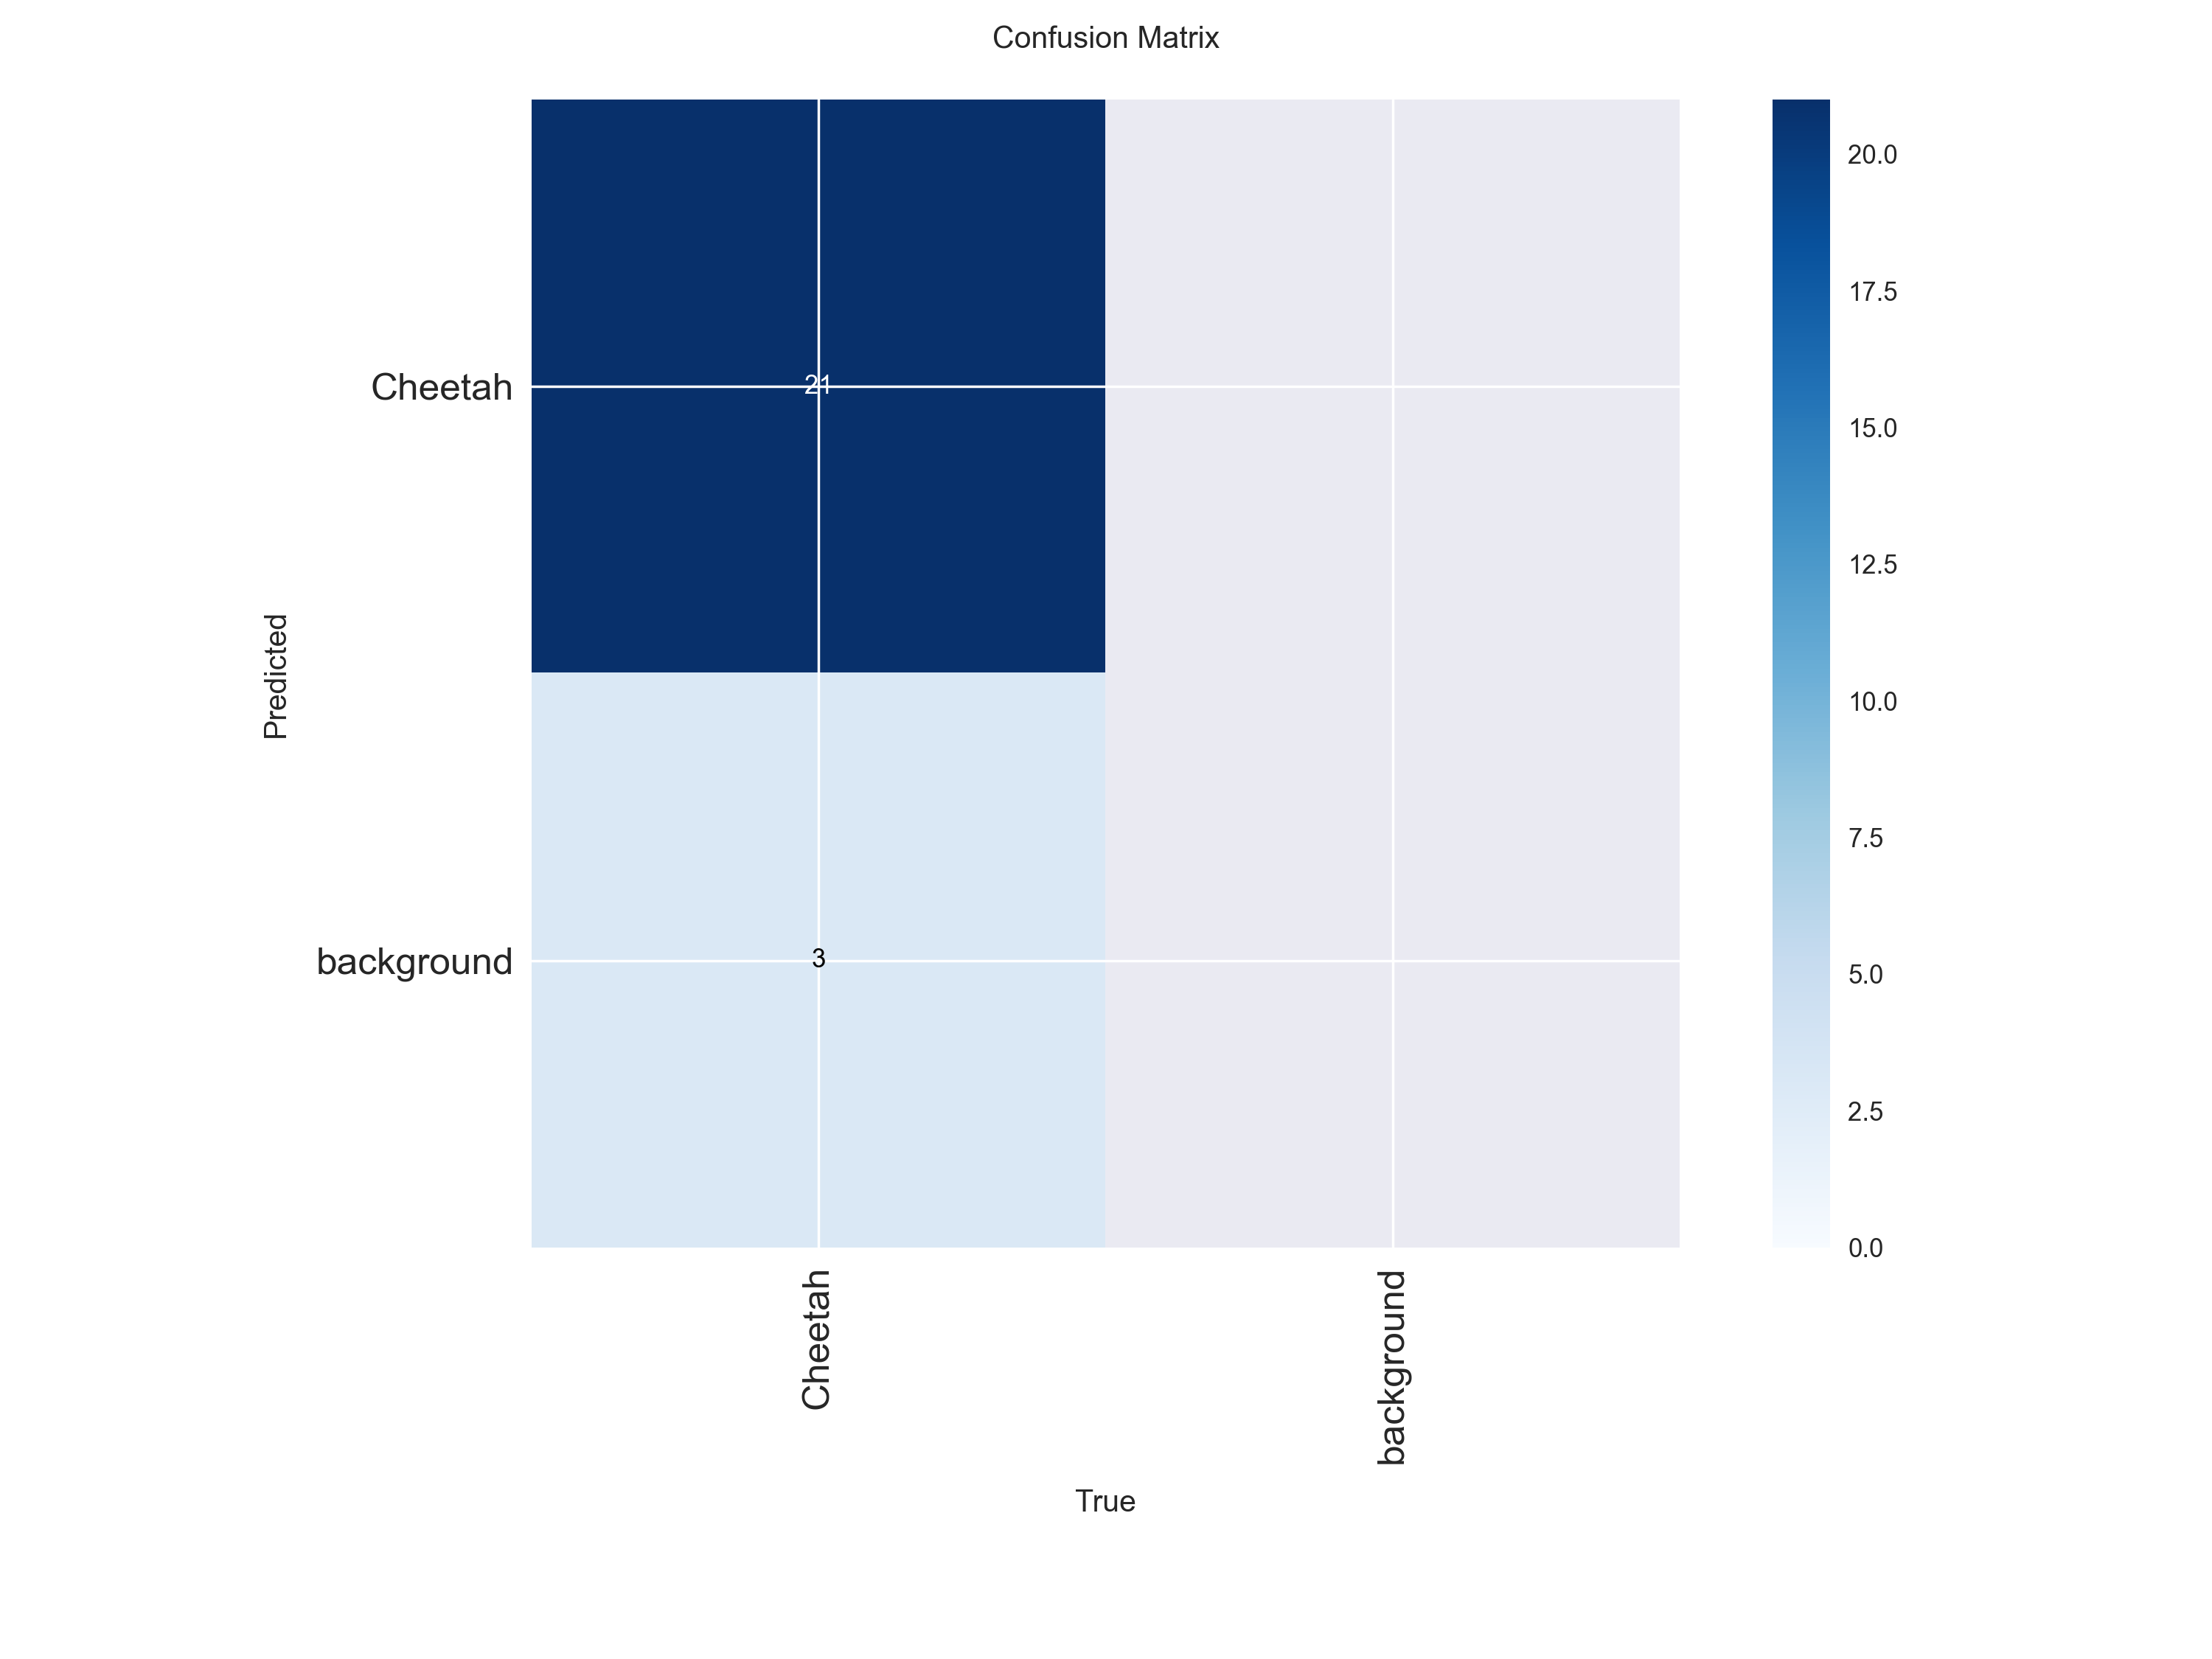
\includegraphics[width=0.35\textwidth]{confusion_matrix.png}}
\caption{Normalized confusion matrix for validation set. The model achieves 87\% true positive rate for cheetah detection with only 12\% false positive rate on background images, demonstrating strong discriminative capability with minimal false detections.}
\label{fig:confusion}
\end{figure}

Figure \ref{fig:validation_batch} shows predictions on a validation batch. All 16 images showed successful detection with confidence 0.9–1.0 across varied poses, occlusion, multiple cheetahs, and lighting conditions.

\begin{figure}[htbp]
\centerline{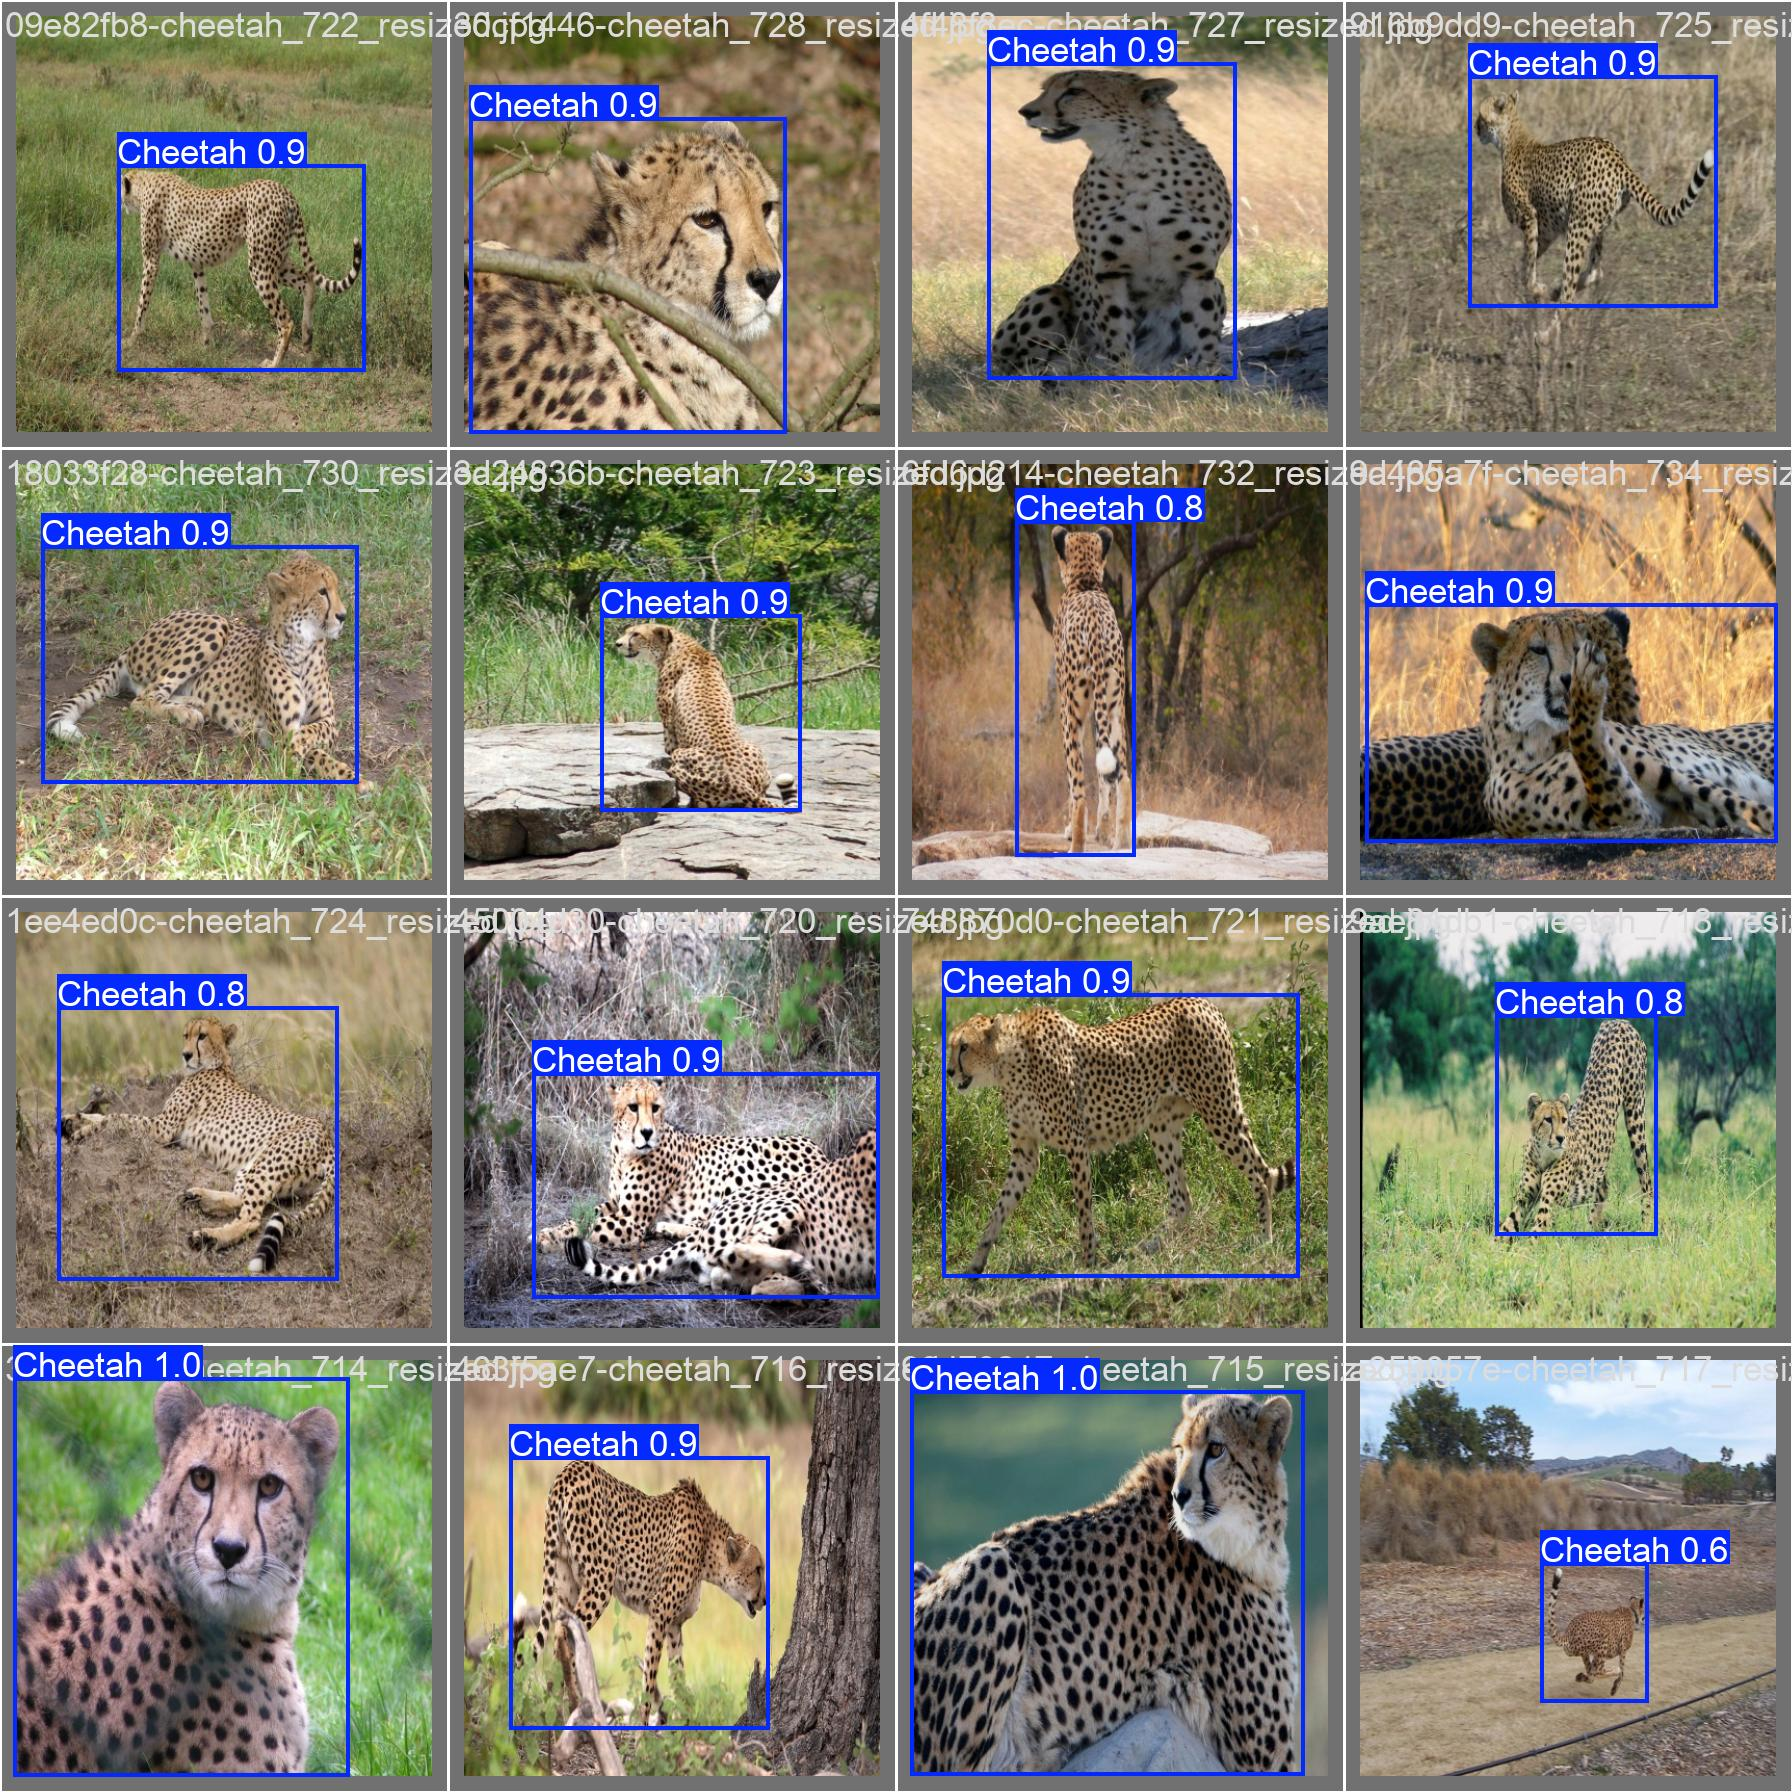
\includegraphics[width=0.45\textwidth]{validation_predictions.png}}
\caption{Validation batch predictions showing detected cheetahs across various poses and environments. All 16 validation images show successful detection with high confidence scores (0.9-1.0), demonstrating robust performance across diverse scenarios including close-up views, partial occlusion, multiple cheetahs, and varied lighting conditions.}
\label{fig:validation_batch}
\end{figure}

Together, these analyses confirm strong single-object performance and reliable positive predictions, while emphasizing limited generalization on complex multi-object scenes.

\section{Critical Analysis and Conclusion}

Strong results were achieved in single-cheetah detection, but reaching these results required extensive fine-tuning and experimentation across multiple training runs. Numerous trials were conducted varying batch sizes (16 to 95), epochs (30 to 100), and hyperparameters before settling on the optimal configuration. The model performs well in live detection scenarios including video inference, maintaining high confidence scores across diverse poses, lighting conditions, and partial occlusion, demonstrating practical utility for wildlife monitoring applications with minimal computational overhead at inference time.

Several limitations emerged during development. Training required an RTX 4060 GPU, and achieving optimal performance necessitated large batch sizes (95) that many standard hardware configurations cannot support. Determining the optimal hyperparameter combination (batch=95, epochs=100, loss weights, confidence thresholds) required analyzing results from over 20 distinct training runs, consuming significant computational resources and development time. The model fails on multi-cheetah scenes (0\% accuracy) with default parameters. While manual parameter tuning (image size and confidence threshold) achieved successful multi-object detection for specific images, this approach lacks generalizability and requires case-by-case optimization. Additionally, the model requires precise threshold selection (confidence=0.35, IoU=0.55) to achieve optimal performance, limiting deployment flexibility. Insufficient training data (379 images) constrained effective generalization for complex scenarios like multiple overlapping animals or varied occlusions.

Future improvements should focus on dataset expansion and automated hyperparameter optimization. Expanding the training dataset to include more diverse multi-cheetah scenes, varied environmental conditions, and synthetic augmentation would improve generalization. Implementing automated hyperparameter tuning using neural architecture search or Bayesian optimization could reduce the time-intensive manual experimentation required in this study. Specifically, training a smaller CNN model to predict optimal training parameters (learning rates, batch sizes, loss weights) based on dataset characteristics could accelerate configuration discovery. Additionally, incorporating k-means clustering for anchor box generation could improve detection accuracy for objects with non-standard aspect ratios. Architectural modifications could address multi-object detection limitations: integrating attention mechanisms to handle occlusions, implementing hierarchical detection for crowded scenes, or designing specialized heads for scale-variant wildlife detection. Deployment improvements should focus on model compression techniques (quantization, pruning) to enable edge device deployment while maintaining accuracy.

This study evaluated YOLOv12-nano for cheetah detection, achieving strong single-object performance (94.6\% accuracy, zero false positives) but revealing critical limitations in multi-object scenarios. The extensive hyperparameter experimentation required substantial computational resources and time investment. While mAP metrics (precision=0.8809, recall=0.7083, mAP@0.5=0.8201) demonstrated strong mathematical performance, custom evaluation based on expected versus actual detections revealed significant gaps across three key scenarios: tiger false positives (expected 0, achieved 0 with extensive tuning), single-cheetah accuracy (expected 1, achieved 94.6\%), and multi-cheetah detection (expected multiple, achieved 0\% with default parameters). The model's effectiveness in live video inference validates practical deployment potential for wildlife monitoring applications. Future work should prioritize automated hyperparameter optimization, dataset diversity, and improved evaluation metrics that align mathematical accuracy with practical detection expectations.

\begin{thebibliography}{00}
\bibitem{b1} J. Redmon, S. Divvala, R. Girshick, and A. Farhadi, ``You Only Look Once: Unified, Real-Time Object Detection,'' in Proc. IEEE Conf. Comput. Vis. Pattern Recognit., Las Vegas, NV, USA, 2016, pp. 779--788, doi: 10.1109/CVPR.2016.91.
\bibitem{b2} J. Redmon and A. Farhadi, ``YOLO9000: Better, Faster, Stronger,'' in Proc. IEEE Conf. Comput. Vis. Pattern Recognit., Honolulu, HI, USA, 2017, pp. 7263--7271, doi: 10.1109/CVPR.2017.690.
\bibitem{b3} A. Aybilge Murat and M. S. Kiran, ``A comprehensive review on YOLO versions for object detection,'' Eng. Sci. Technol., an Int. J., vol. 70, 2025, p. 102161, doi: 10.1016/j.jestch.2025.102161.
%%% MORE REFERENCES TO BE ADDED - Need to add papers for YOLO evolution, object detection, transfer learning %%%
\end{thebibliography}

\end{document}